\documentclass[handout]{beamer} % add [handout] to collapse \pause-s
\usetheme{default}
\usepackage{array}
%\usepackage{amsmath}
\usepackage{mathtools}
\usepackage{hyperref}
\usepackage{pdfpages}

\usepackage{alltt}
\usepackage{color}
\definecolor{string}{rgb}{0.7,0.0,0.0}
\definecolor{comment}{rgb}{0.13,0.54,0.13}
\definecolor{keyword}{rgb}{0.0,0.0,1.0}

\newcommand{\br}{\vspace{\baselineskip}}

\beamertemplatenavigationsymbolsempty

\title{The Parts and Compositors Framework}
\subtitle{Using MATLAB and ODEs to understand the behavior of multi-part systems}
\author[kristjan@mit.edu]{(Kristjan) Eerik Kaseniit (eerik@mit.edu),
Jacob Becraft (jbecraft@mit.edu)}
\institute[MIT]{
	Massachusetts Institute of Technology \\
	20.305 Principles of Synthetic Biology
}
\date{September 25, 2014}

\usepackage{graphicx}
\begin{document}

\begin{frame}[plain]
  \titlepage
  
  \begin{center}\href{http://web.mit.edu/20.305/www/tutorial/}{http://web.mit.edu/20.305/www/tutorial/}\end{center}
\end{frame}

\begin{frame}{Differential equations -- the usual tool}

\begin{itemize}
\item What are they?

Equations relating variables with their derivatives.

\pause

Examples:

\hspace{23 mm}\emph{Differentiation} $\rightarrow$

\hspace{23 mm}$\leftarrow$ \emph{Integration}

\renewcommand{\arraystretch}{1.5}
\begin{tabular}{m{0.4\textwidth}m{0.4\textwidth}}
	\emph{Equation} & \emph{Differential equation} \\
	$ x(t) = c $ & $ \dot x = 0 \onslide<3->{\Leftrightarrow \frac{dx}{dt} = 0} $ \\
	\pause
	\pause
	$ x(t) = ct + d $ & $ \dot x = c $ \\
	\pause
	$ x(t) = ct^2 + d $ & $ \dot x = 2ct $ \\
\end{tabular}

\pause

\vspace{7 mm}

This is all pretty ''mathematical''. How can we use diff eqs to describe biological processes, chemical reactions?

\end{itemize}

\end{frame}


\begin{frame}{Setting up differential equations}

\begin{itemize}

\item Let's consider a chemical reaction:
\pause
$$ E + S \xrightleftharpoons[k_r]{k_f} ES $$
\pause
Reaction: an enzyme $E$ binds a substrate $S$ to form an enzyme-substrate complex $ES$.
\pause
\item Three species in this system, so we'll have three equations describing their \emph{concentrations} changing over time:
$$ \frac{d[E]}{dt} = \onslide<5->{-k_f [E][S] + k_r[ES]} $$
$$ \frac{d[S]}{dt} = \onslide<5->{-k_f [E][S] + k_r[ES]} $$
$$ \frac{d[ES]}{dt} = \onslide<5->{k_f [E][S] - k_r[ES]} $$
\pause
\pause
What are the units of $[E], d[S]/dt, k_f, k_r$?
\end{itemize}

\end{frame}

\begin{frame}{Reading a differential equation}

$$ \frac{d[ES]}{dt} = k_f [E][S] - k_r[ES] $$

\begin{itemize}
	\item \emph{What are we describing?}\\ \pause
	The rate of change of the concentration of $ES$. \pause
	\item \emph{How many molecules come together to form $ES$?}\\ \pause
	There are two concentration terms in the forward reaction -- so two. \pause
	\item \emph{Suppose that a second substrate molecule must be present for the complex to form -- how would the equation change?}\\ \pause
	It would be $ d[ES]/dt = k_f'[E][S]^\mathbf{2} - k_r'[ES_2] $\pause
	\item \emph{What increases the rate of change?}\\ \pause
	Increasing $k_f, [E], [S]$; decreasing $k_r, [ES]$. \pause
\end{itemize}

\end{frame}

\begin{frame}{Predicting using a differential equation}

$$ \frac{d[ES_n]}{dt} = k_f [E][S]^n - k_r[ES_n] $$

\begin{itemize}

	\item Suppose we start with no $ES_n$, $[E](t = 0) = [E]_0$, $[S](t = 0) = [S]_0$ and we don't make any new $E, S$. After long enough time, what is the \emph{steady-state concentration} of $ES_n$? \pause
	
	\vspace{3 mm}
	
	Hint: Steady-state $\Rightarrow$ rate of change is zero. \pause

\end{itemize}

\end{frame}


\begin{frame}{Predicting using a differential equation}
	$$ \frac{d[ES_n]}{dt} = k_f [E][S]^n - k_r[ES_n] $$
	$$ \frac{d[ES_n]}{dt} = 0 \Rightarrow k_f[E][S]^n = k_r[ES_n] $$ \pause
	$$ [ES_n] = \frac{k_f}{k_r} [E][S]^n $$ \pause
	Is this it? \pause What are $[E], [S]$? \pause Set:
	$$ [E]_{total} = [E] + [ES_n], ~~~ [S]_{total} = [S] + [ES_n] \approx [S] \text{ (if } [S]_0 \gg [E]_0) $$ \pause % TODO: check!
	\vspace{-2.5mm}
	$$ \frac{k_r}{k_f} [ES_n] = ([E]_{total} - [ES_n])[S]_{total}^n $$ \pause
	$$ [ES_n] \left ( \frac{k_r}{k_f} - [S]_{total}^n \right ) = [E]_{total} [S]_{total}^n $$ \pause
	$$ \boxed{ [ES_n]_{steady-state} = \frac{[S]_{total}^n}{\frac{k_r}{k_f} - [S]_{total}^n} [E]_{total} }$$
\end{frame}

\begin{frame}{Predicting using a differential equation}
	$$ [ES_n]_{steady-state} = \frac{[S]_{total}^n}{\frac{k_r}{k_f} - [S]_{total}^n} [E]_{total} $$
	But $[E]_{total} = E_0, [S]_{total} = S_0$: \pause
	$$ [ES_n]_{steady-state} = \frac{[S]_0^n}{\frac{k_r}{k_f} - [S]_0^n} [E]_0 $$
	\pause
	Hill term: $$ \boxed{\frac{X^n}{K^n + X^n}} $$
	\pause
	$n$ -- "cooperativity", Hill coefficient; $K$ -- a characteristic constant ($X$ at which the fraction is $1/2$)

	\pause
	Limits as $X \rightarrow 0$ or $X \rightarrow \infty$? \pause 0, 1.
\end{frame}

\begin{frame}{Describing a biological system}

\pause

\textbf{The Central Dogma!} \pause

\vspace{5 mm}

\hspace{27 mm} \hspace{21 mm} $\emptyset$ \hspace{15 mm} $\emptyset$

\hspace{27 mm} \hspace{21 mm} $\uparrow k_{mdeg}$ \hspace{5 mm} $\uparrow k_{pdeg}$ 

\hspace{27 mm} DNA $\xrightarrow{k_{txn}}$ mRNA $\xrightarrow{k_{tln}}$ Protein

\pause

\emph{Note: this is more of a diagram than a set of equations.}

\pause

\vspace{2 mm}

$$ \frac{d[mRNA]}{dt} = k_{txn}[DNA] - k_{mdeg}[mRNA] $$
$$ \frac{d[Protein]}{dt} = k_{tln}[mRNA] - k_{pdeg}[Protein] $$

\pause

\vspace{5 mm}

\emph{What are we leaving out?} \pause E.g. no cell division (dilution \& replication), are neglecting small-number effects.

\end{frame}

\begin{frame}{Something more interesting: modeling a repressor}

Step 1: Model repressor-DNA binding.

\emph{Sounds a bit like enzyme-substrate binding...?}

\vspace{2 mm}

Step 2: Apply central dogma.

\emph{Ah! I know this!}

\end{frame}

\begin{frame}{Modeling a repressor: repressor-DNA binding}

$$ nR + DNA \xrightleftharpoons[k_r]{k_f} R_n:DNA $$ \pause

If we assume that equilibrium is achieved rapidly (not unreasonable), then we are at steady-state conditions:

$$ \frac{d[R_n:DNA]}{dt} = 0 $$ \pause
Thinking back to enzyme-substrate binding, we say that $[DNA] \ll [R]$ and so:
$$ [R_n:DNA] = \frac{[R]^n}{K^n + [R]^n} [DNA] ~~~~ \pause K = (k_r / k_f)^{1/n} $$\pause

Note: because of the assumption above, the "enzyme" is the DNA and the "substrate" is the repressor if we think about the equations. \pause $n=2$ means roughly that the repressor dimerizes.

\end{frame}

{
\setbeamercolor{background canvas}{bg=}
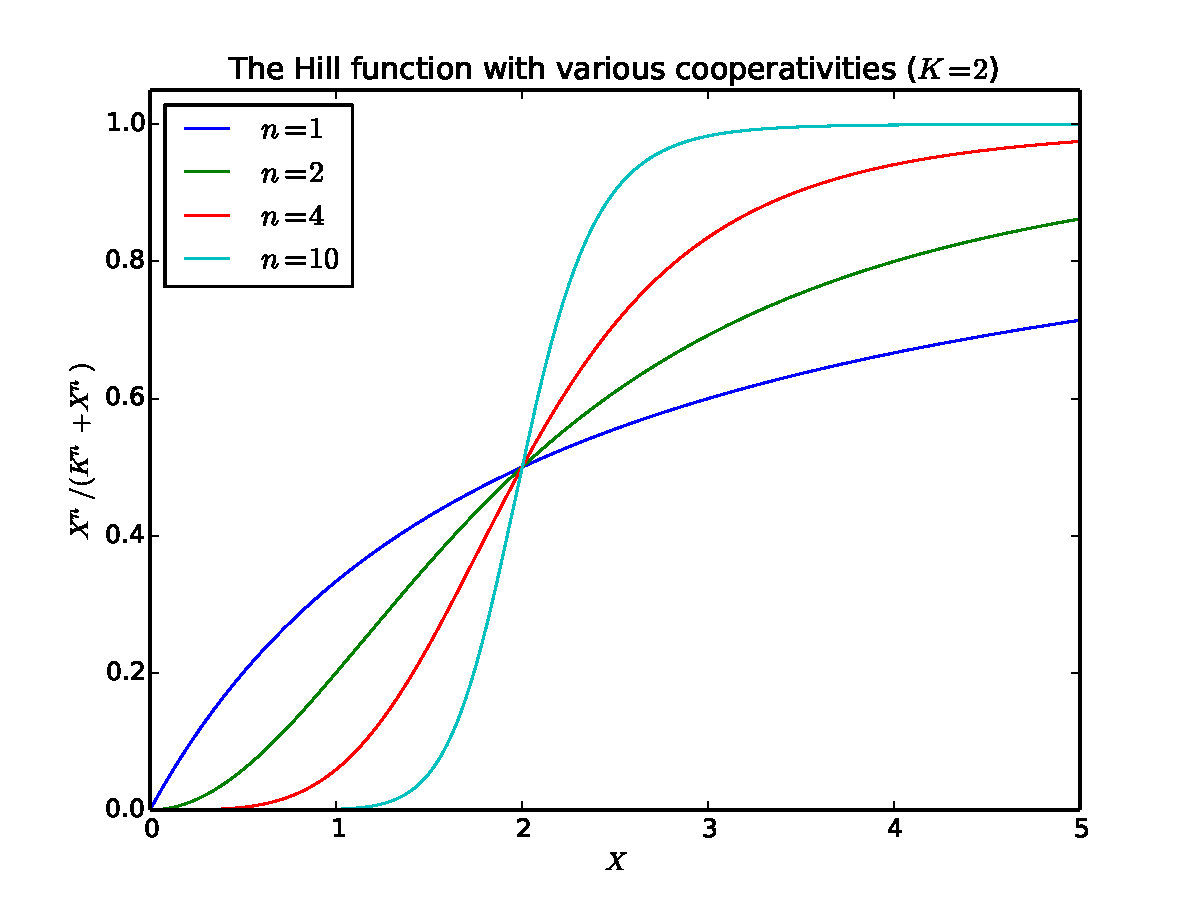
\includepdf[pages=1]{Hill.pdf}
}

\begin{frame}{Modeling a repressor: relating to central dogma}

Only DNA \emph{not} bound the repressor can be transcribed:

$$ \frac{d[mRNA]}{dt} = k_{txn}[DNA]_{tot}\left ( 1 - \frac{[R]^n}{K^n + [R]^n} \right ) - k_{mdeg}[mRNA] $$

\pause \hspace{37 mm}\emph{Fraction not bound by repressor}

\end{frame}

{
\setbeamercolor{background canvas}{bg=}
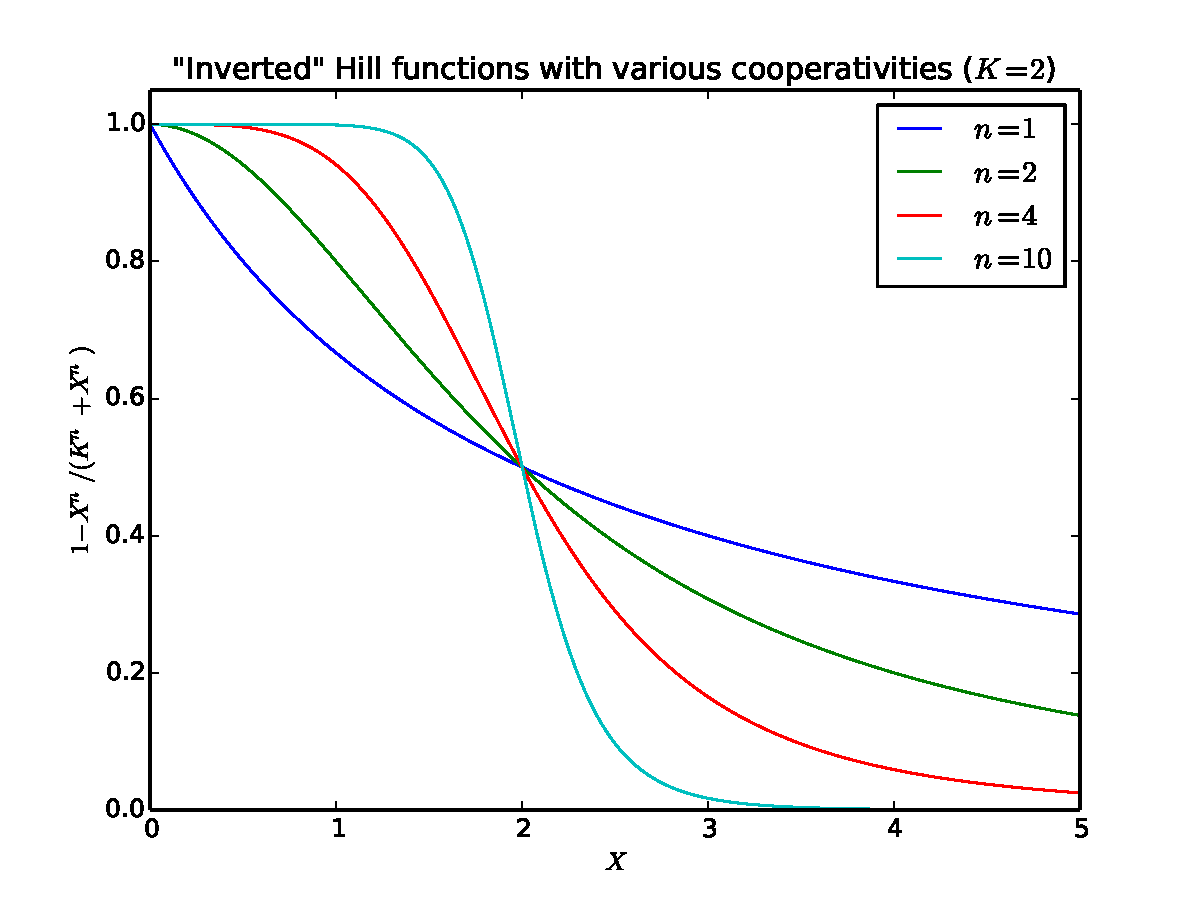
\includepdf[pages=1]{NOTHill.pdf}
}

\begin{frame}{Extending the model -- how to describe the requirement for activation?}

\pause

Hint:

\begin{center}\begin{tabular}{cc|c|c}
	$A$ & $B$ & $A$ AND $B$ & $A \cdot B$ \\ \hline
	0 & 0 & 0 & 0\\
	0 & 1 & 0 & 0\\
	1 & 0 & 0 & 0\\
	1 & 1 & 1 & 1\\
\end{tabular}\end{center}

\pause

$$ \frac{d[mRNA]}{dt} = k_{txn}[DNA]_{tot}\left ( 1 - \frac{[R]^{n_R}}{K_R^{n_R} + [R]^{n_R}} \right ) \cdot \left ( \frac{[A]^{n_A}}{K_A^{n_A} + [A]^{n_A}} \right ) $$$$- k_{mdeg}[mRNA] $$

\end{frame}

\begin{frame}{Numerical analysis of differential equations}

Most interesting diff eqs are hard to solve analytically. This leaves two common options: \pause
\begin{itemize}
	\item Numerical integration \pause
	
	Start with some initial conditions, and integrate little-by-little. E.g. \texttt{ode23s} in MATLAB. \pause
	
	\item Stochastic simulations \pause
	
	Reaction rates are like probabilities: throw weighted dice to figure out a) when the next reaction is happening and b) which one from a set of reactions occurs. E.g. Gillespie algorithm.
\end{itemize}

\end{frame}

\begin{frame}{MATLAB tips and tricks}
\begin{itemize}
    \item Use up/down arrows to navigate history (Ctrl-R to search)
    \item Use \texttt{;} at the end of a statement to suppress output
    \item \texttt{disp('a')} will print out \texttt{a} (can use variables)
    \item \texttt{clear all} will clear the workspace, \texttt{clc} just the screen
    \item MATLAB over SSH from Athena: \texttt{ssh -XC -c blowfish -l YOUR\_KERBEROS athena.dialup.mit.edu} (might need \href{http://xquartz.macosforge.org/landing/}{XQuartz} for Macs)
    \item \texttt{help sqrt} will bring up the manual for the $\sqrt{}$ function
    \item \texttt{lookfor square} will search for "square" in docs ($\sim$ slow)
    \item \texttt{f = @(x) (x\^{}2)} creates an "anonymous" function in a script,
        call e.g. \texttt{f(2)}
    \item \texttt{hold on} adds \texttt{plot()} results to current figure; \texttt{hold all} will also use new color/style automatically
    \item \texttt{ans} holds result of last statement
\end{itemize}
\end{frame}


\begin{frame}{MATLAB tips and tricks}
\begin{itemize}
    \item \texttt{[1:5] == [1 2 3 4 5]}
    \item \texttt{A'} will transpose \texttt{A}
    \item \texttt{[1:5]' == [1; 2; 3; 4; 5]}
    \item \texttt{A(:, 2)} gives the second column of the matrix \texttt{A}
    \item \texttt{A(:, end)} gives the last column of the matrix \texttt{A}
    \item \texttt{...} lets you break up long lines
    \item Look at the \texttt{.m} files that make up our framework!
    
    They're short :)
\end{itemize}
\end{frame}

\begin{frame}[fragile]{Setup for the part-compositor framework}

To download the part-compositor framework, run this once in MATLAB in
your work directory:

\begin{verbatim}
urlwrite(['http://web.mit.edu/20.305/www/' ...
    'part_composition_setup.m'], ...
    'part_composition_setup.m');
rehash;
part_composition_setup('v2pre');
\end{verbatim}

\pause

Note: for problem submissions, you must include this sort of statement at the top of the
problem (always given in the problem template)

\pause

\br
To download the scripts we will be looking at here, go to \texttt{http://web.mit.edu/20.305/www/tutorial/}

\pause

\br
Off we go!

\end{frame}




\begin{frame}{Parts are processes and compositors help connect them}

Parts are processes

\begin{itemize}
	\item \textbf{Inputs}: a subset of state variables
	\item \textbf{Outputs}: a set of rates of change of a possibly overlapping set of other state variables
\end{itemize}

\pause

Compositors aggregate effects of parts

\begin{itemize}
	\item There is one compositor for each state variable of the system
	\item Multiple parts may act on the same state variable and thus on the compositor \pause
	\item \textbf{Inputs}: certain rates from possibly many parts (to produce a change in the relevant state variable)
	\item \textbf{Output}: the state variable \pause
	\item We call compositors by their state variable name
\end{itemize}

\end{frame}

\begin{frame}{Example from class}

\textbf{Part}: conversion of $M_1 \rightarrow M_2$ mediated by $E_1$ with rate law $k_{cat} [E_1] \frac{[M_1]}{K_m + [M_1]}$

\pause
\br

\textbf{Compositors}:\pause $\frac{d[E_1]}{dt}$ (named \texttt{E1}), $\frac{d[M_1]}{dt}$ (\texttt{M1}), $\frac{d[M_2]}{dt}$ (\texttt{M2})\pause
$$ v_{E_1}^1 = \frac{d[E_1]}{dt} = \pause0 $$
$$ v_{M_1}^1 = \frac{d[M_1]}{dt} = \pause- k_{cat} [E_1] \frac{[M_1]}{K_m + [M_1]} $$
$$ v_{M_2}^1 = \frac{d[M_2]}{dt} = \pause  k_{cat} [E_1] \frac{[M_1]}{K_m + [M_1]} $$

\pause

%\br
\textbf{Initial conditions}:
$$ [E_1] (t = 0~s) = 10~\mu M$$
$$ [M_1] (t = 0~s) = 10~\mu M$$
$$ [M_2] (t = 0~s) = 0~\mu M$$

\end{frame}

\begin{frame}[fragile]{Coding it up in MATLAB}

\textbf{Part}: conversion of $M_1 \rightarrow M_2$ mediated by $E_1$ with rate law $k_{cat} [E_1] \frac{[M_1]}{K_m + [M_1]}$

\fontsize{0.75em}{0.75em}
\begin{alltt}
0001 sys1 = BioSystem();\pause
0002 
0003 \textcolor{comment}{% create compositors, set initial state}
0004 E1 = Compositor(\textcolor{string}{'E1'}, 10); \textcolor{comment}{% units implied}
0005 M1 = Compositor(\textcolor{string}{'M1'}, 10);
0006 M2 = Compositor(\textcolor{string}{'M2'}, 0);\pause
0007 
0008 sys1.AddCompositor(E1);
0009 sys1.AddCompositor(M1);
0010 sys1.AddCompositor(M2);\pause
0011 
0012 sys1.AddConstant(\textcolor{string}{'k_cat'}, 10); \textcolor{comment}{% units implied}
0013 sys1.AddConstant(\textcolor{string}{'K_m'}, 5);\pause
0014 
0015 P1 = Part(\textcolor{string}{'M1-(E1)->M2'}, [M1 E1 M2], \textcolor{keyword}{\underline{...}}\pause
0016           [ Rate(\textcolor{string}{'- k\_cat * E1 * (M1 / (K\_m + M1))'}) \textcolor{keyword}{\underline{...}}\textcolor{comment}{ \% M1}\pause
0017             Rate(\textcolor{string}{'0'}), \textcolor{keyword}{\underline{...}}\textcolor{comment}{ \% E1}\pause
0018             Rate(\textcolor{string}{'  k\_cat * E1 * (M1 / (K\_m + M1))'}) \textcolor{keyword}{\underline{...}}\textcolor{comment}{ \% M2}
0019           ]);\pause
0020  
0021 sys1.AddPart(P1);\pause
0022 
0023 [T, Y] = sys1.run([0 3]) \textcolor{comment}{% units implied}
0024 plot(T, Y)
\end{alltt}

\end{frame}

\begin{frame}{How can \emph{I} run it?}
\pause
Go to the folder where you've downloaded the framework as well as \texttt{sys1\_simple\_enzyme.m}

\pause
\br

Then in your prompt:

\texttt{>>\pause~ sys1\_simple\_enzyme}

\end{frame}

\begin{frame}{}

\begin{figure}[htp]
    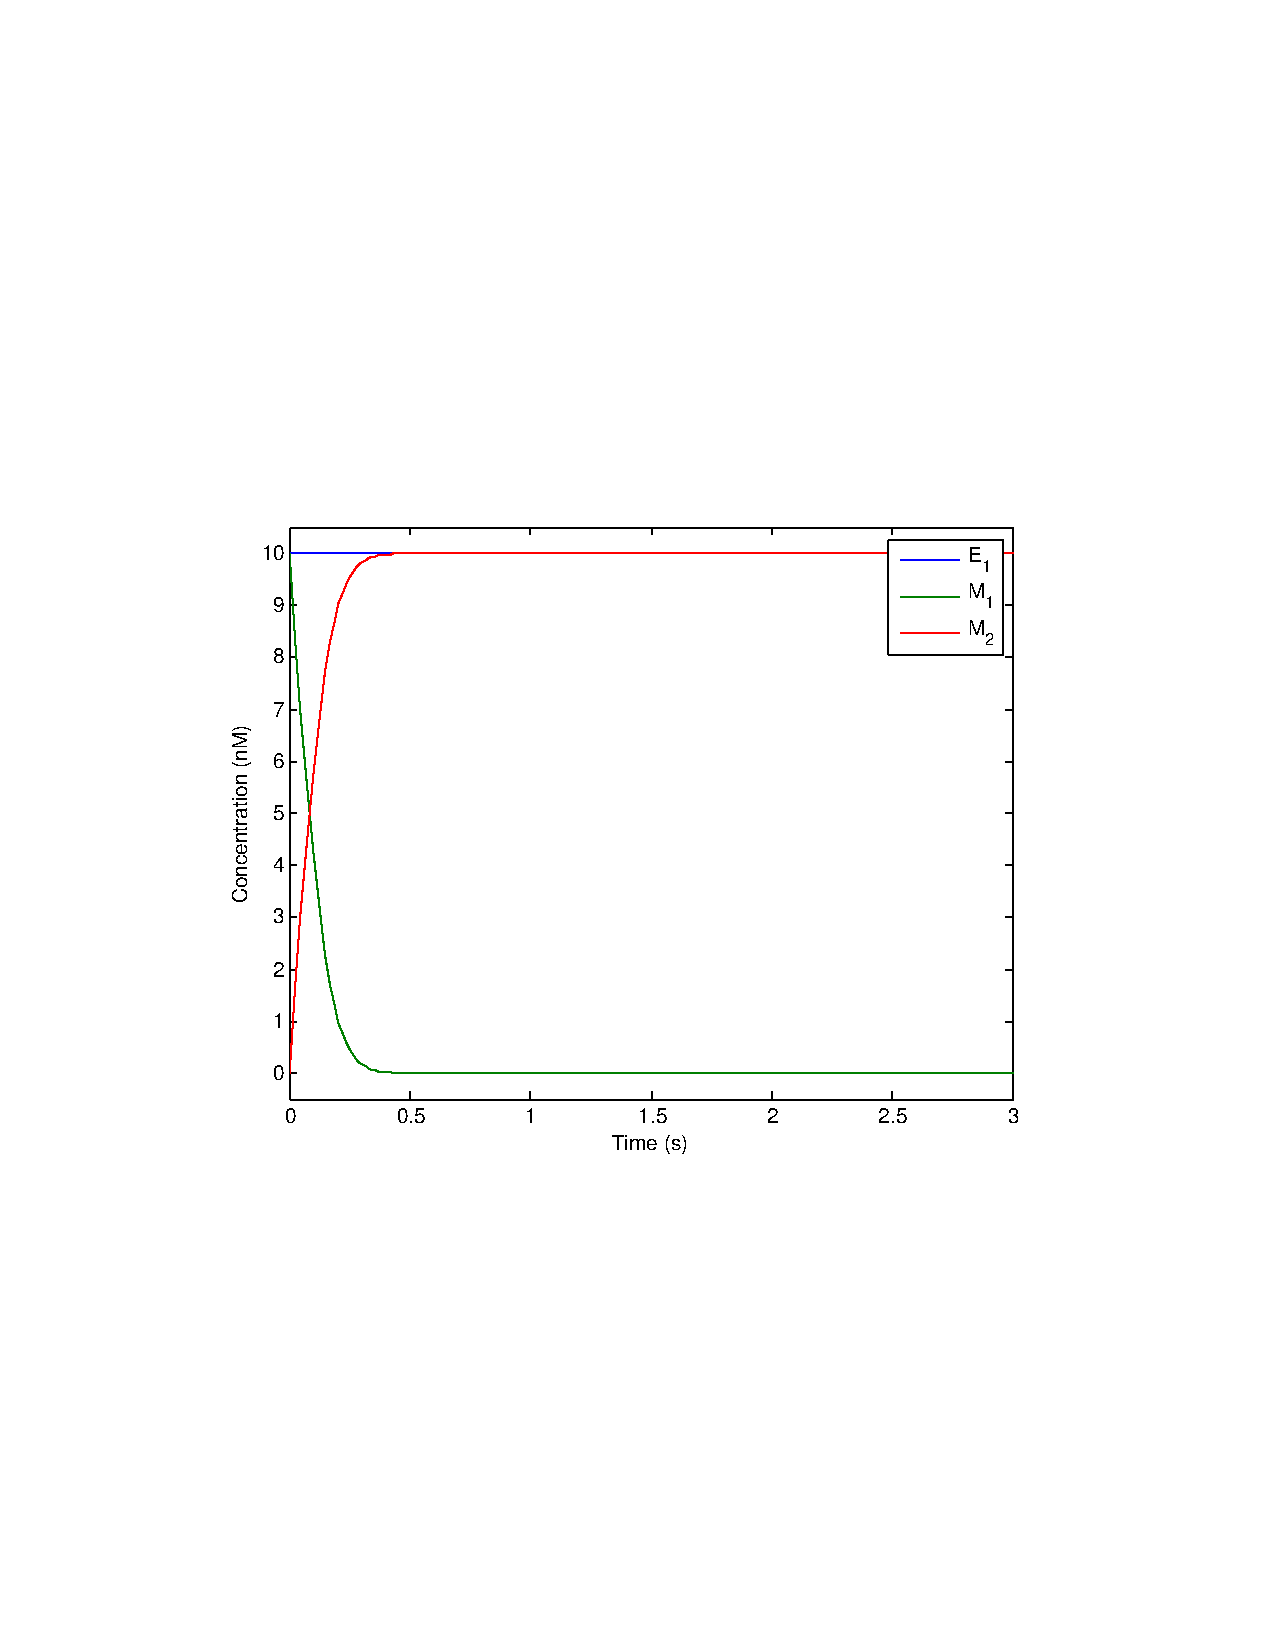
\includegraphics[scale=0.65, clip=true, trim=3.5cm 8cm 3.5cm 8cm]{sys1.pdf}
\end{figure}

\end{frame}

\begin{frame}{A mystery part in a new system}

\textbf{Part}: a mystery process involving a single state variable, $x$. The behavior of $x$ is governed by the equation
$$ \frac{d^2x}{dt^2} - \mu (1 - x^2)\frac{dx}{dt} + x = 0 $$

This state variable starts off with $x(0) = 1, \dot x = 0.5$

\pause
\br

\textbf{Compositors}:\pause ~?!? how do I define a compositor when we take second derivatives ?!?\pause

Answer:\pause ~Substitution! use $y = \dot x$\pause

Now we have a state variable that's not a physical thing, but that's OK, it's all make-believe anyway!\pause

$$v_{x}^1 = \frac{dx}{dt} = y$$
$$\frac{dy}{dt} - \mu (1 - x^2)y + x = 0 \Rightarrow v_{y}^1 = \frac{dy}{dt} = \mu (1 - x^2)y - x $$

\end{frame}

\begin{frame}[fragile]{Simulating our mystery part}

$$v_{x}^1 = y$$
$$v_{y}^1 = \mu (1 - x^2)y - x $$

\fontsize{0.75em}{0.75em}
\begin{alltt}
0001 sys2 = BioSystem();\pause
0002 
0003 x = sys2.AddCompositor(\textcolor{string}{'x'}, 1);
0004 y = sys2.AddCompositor(\textcolor{string}{'y'}, 0.5);\pause
0005 
0006 sys2.AddConstant(\textcolor{string}{'mu'}, 5);\pause
0007 
0008 sys2.AddPart(Part(\textcolor{string}{'Van der Pol wibbly-wobbly-timey-wimey'}, [x y], \textcolor{keyword}{\underline{...}}\pause
0009     [ Rate(\textcolor{string}{'y'}) \textcolor{keyword}{\underline{...}}\textcolor{comment}{ \% x}\pause
0010       Rate(\textcolor{string}{'mu * (1 - x\^{}2) * y - x'}), \textcolor{keyword}{\underline{...}}\textcolor{comment}{ \% y}
0011     ]));
0012 
0013 figure();
0014 hold all; \textcolor{comment}{% plot() will use same figure, different colors}
0015 time\_interval = [0 80];\pause
0016 \textcolor{keyword}{for} mu = [0 5 25]
0017     sys2.ChangeConstant(\textcolor{string}{'mu'}, mu)
0018     [T, Y] = sys2.run(time\_interval);
0019     plot(T, Y(:, 1))
0020 \textcolor{keyword}{end}\pause
0021 legend(\textcolor{string}{'\(\backslash\)mu = 0'}, \textcolor{string}{'\(\backslash\)mu = 5'}, \textcolor{string}{'\(\backslash\)mu = 25'})
0022 xlabel(\textcolor{string}{'Time'})
0023 ylabel(\textcolor{string}{'Value'})
\end{alltt}

\end{frame}

\begin{frame}{What does this wibbly-wobbly-timey-wimey part do then?!}
\pause
\begin{figure}[htp]
    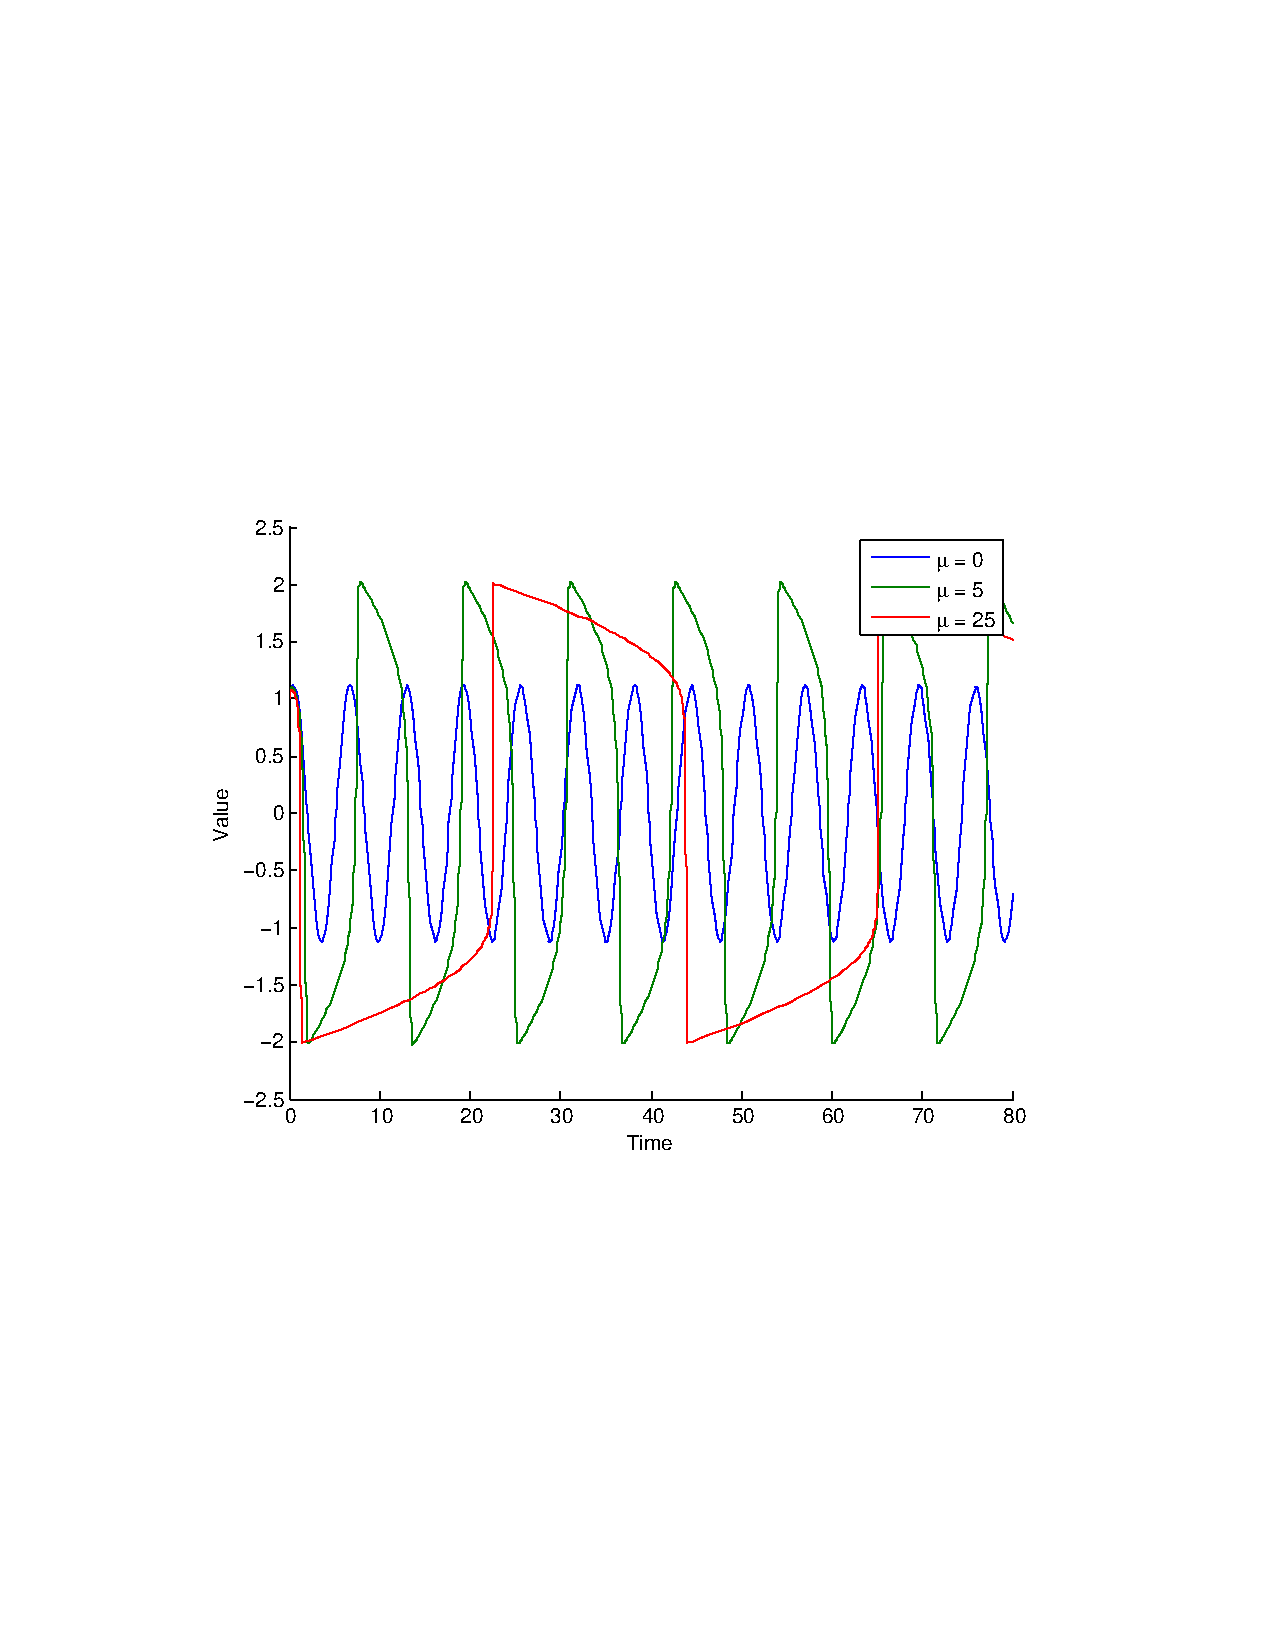
\includegraphics[scale=0.60, clip=true, trim=3.5cm 8cm 3.5cm 8cm]{sys2.pdf}
\end{figure}

\end{frame}

\begin{frame}{Ah, I want a wibbly-wobbly-timey-wimey thing!}

You're in luck! There are many ways to implement oscillators using gene-regulatory elements.

\pause
\br
Here's one way ("activator-inhibitor" topology):
\begin{figure}
    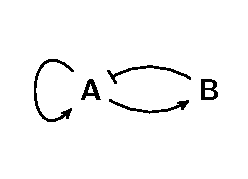
\includegraphics[scale=1]{hasty_diagram.pdf}
\end{figure}

\pause A circuit with this abstract topology was implemented e.g. by Stricker \emph{et al.} (Nature 2008), Prindle \emph{et al.} (Nature 2012, \href{http://go.nature.com/lrOtKQ}{http://go.nature.com/lrOtKQ})

\end{frame}

\begin{frame}{Decomposing the activator-inhibitor topology}
\begin{figure}
    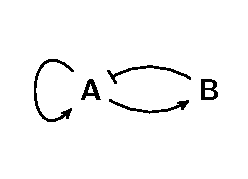
\includegraphics[scale=1]{hasty_diagram.pdf}
\end{figure}

\textbf{Parts}: \pause transcription of $A, B$, translation of $A, B$, degradation of $A, m_A, B, m_B$

\br

\textbf{Compositors}: \pause $\frac{dm_A}{dt}, \frac{dm_B}{dt}, \frac{dA}{dt}, \frac{dB}{dt}$ \pause

\br

\textbf{General model}: fraction of promoter bound by $X$ is given by $\frac{X^n}{X^n + K_x^n}$ where $K_X$ is the concentration of $X$ where the fraction bound is 0.5 and $n$ is a characteristic constant, roughly how many molecules of $X$ come together before binding.


\end{frame}

\begin{frame}{Writing out the rates for parts in the activator-inhibitor topology}
\begin{figure}
    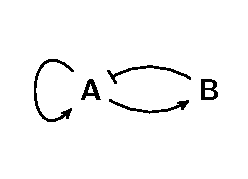
\includegraphics[scale=1, clip=true, trim=0 0.9cm 0 1cm]{hasty_diagram.pdf}
\end{figure}

\textbf{Parts}:  transcription of $A, B$ (1-2), translation of $A, B$ (3-4), degradation of $A, m_A, B, m_B$ (5-8)

\br

\textbf{Rates}:

\centering
\begin{tabular}{cc}
	$v_{m_A}^1 = k_{tx} \cdot \frac{A^n}{K_A^n + A^n} \cdot \frac{K_B^n}{K_B^n + B^n}$ \pause & $v_{m_B}^2 = k_{tx} \cdot \frac{A^n}{K_A^n + A^n} \pause $\\
	$v_A^3 = k_{tln} \cdot m_A $ & $v_B^4 = k_{tln} \cdot m_B \pause $\\
	$v_A^5 = - k_{pdeg} \cdot A$ & $v_{m_A}^6 = - k_{mdeg} \cdot m_A $ \\
	$v_B^7 = - k_{pdeg} \cdot B$ & $v_{m_B}^8 = - k_{mdeg} \cdot m_B $ \\
\end{tabular}

\end{frame}

\begin{frame}[fragile]

\fontsize{0.65em}{0.65em}
\begin{alltt}
0001 sys3 = BioSystem();\pause
0002 
0003 A = sys3.AddCompositor(\textcolor{string}{'A'}, 10); mA = sys3.AddCompositor(\textcolor{string}{'mA'}, 1);
0004 B = sys3.AddCompositor(\textcolor{string}{'B'}, 10); mB = sys3.AddCompositor(\textcolor{string}{'mB'}, 1);\pause
0005 
0006 sys3.AddConstant(\textcolor{string}{'k\_tx'}, 5); sys3.AddConstant(\textcolor{string}{'k\_tl'}, 5);
0007 sys3.AddConstant(\textcolor{string}{'k\_mdeg'}, 0.5); sys3.AddConstant(\textcolor{string}{'k\_pdeg'}, 0.05);
0008 sys3.AddConstant(\textcolor{string}{'K\_A'}, 1); sys3.AddConstant(\textcolor{string}{'K\_B'}, 2);
0009 sys3.AddConstant(\textcolor{string}{'n'}, 2);\pause
0010 
0011 sys3.AddPart(Part(\textcolor{string}{'Transcription of A'}, [mA], \textcolor{keyword}{\underline{...}}
0012     [ Rate(\textcolor{string}{'k\_tx * A\^{}n / (K\_A\^{}n + A\^{}n) * K\_B\^{}n / (K\_B\^{}n + B\^{}n)'}) ]));
0013 
0014 sys3.AddPart(Part(\textcolor{string}{'Transcription of B'}, [mB], \textcolor{keyword}{\underline{...}}
0015     [ Rate(\textcolor{string}{'k\_tx * A\^{}n / (K\_A\^{}n + A\^{}n)'}) ]));\pause
0016 
0017 sys3.AddPart(Part(\textcolor{string}{'Translation of A'}, [A], \textcolor{keyword}{\underline{...}}
0018     [ Rate(\textcolor{string}{'k\_tl * mA'}) ]));
0019 sys3.AddPart(Part(\textcolor{string}{'Translation of B'}, [B], \textcolor{keyword}{\underline{...}}
0020     [ Rate(\textcolor{string}{'k\_tl * mB'}) ]));\pause
0021 
0022 sys3.AddPart(Part(\textcolor{string}{'Degradation of A'}, [A], \textcolor{keyword}{\underline{...}}
0023     [ Rate(\textcolor{string}{'- k\_pdeg * A'}) ]));
0024 sys3.AddPart(Part(\textcolor{string}{'Degradation of mA'}, [mA], \textcolor{keyword}{\underline{...}}
0025     [ Rate(\textcolor{string}{'- k\_mdeg * mA'}) ]));
0026 sys3.AddPart(Part(\textcolor{string}{'Degradation of B'}, [B], \textcolor{keyword}{\underline{...}}
0027     [ Rate(\textcolor{string}{'- k\_pdeg * B'}) ]));
0028 sys3.AddPart(Part(\textcolor{string}{'Degradation of mB'}, [mB], \textcolor{keyword}{\underline{...}}
0029     [ Rate(\textcolor{string}{'- k\_mdeg * mB'}) ]));\pause
0030 
0031 figure();
0032 [T, Y] = sys3.run([0 2000]);
0033 plot(T, Y);
0034 legend(\textcolor{string}{'A'}, \textcolor{string}{'m\_A'}, \textcolor{string}{'B'}, \textcolor{string}{'m\_B'});
0035 xlabel(\textcolor{string}{'Time'});
0036 ylabel(\textcolor{string}{'Concentration'});\pause
\end{alltt}
\end{frame}

\begin{frame}
\pause
\begin{figure}[htp]
    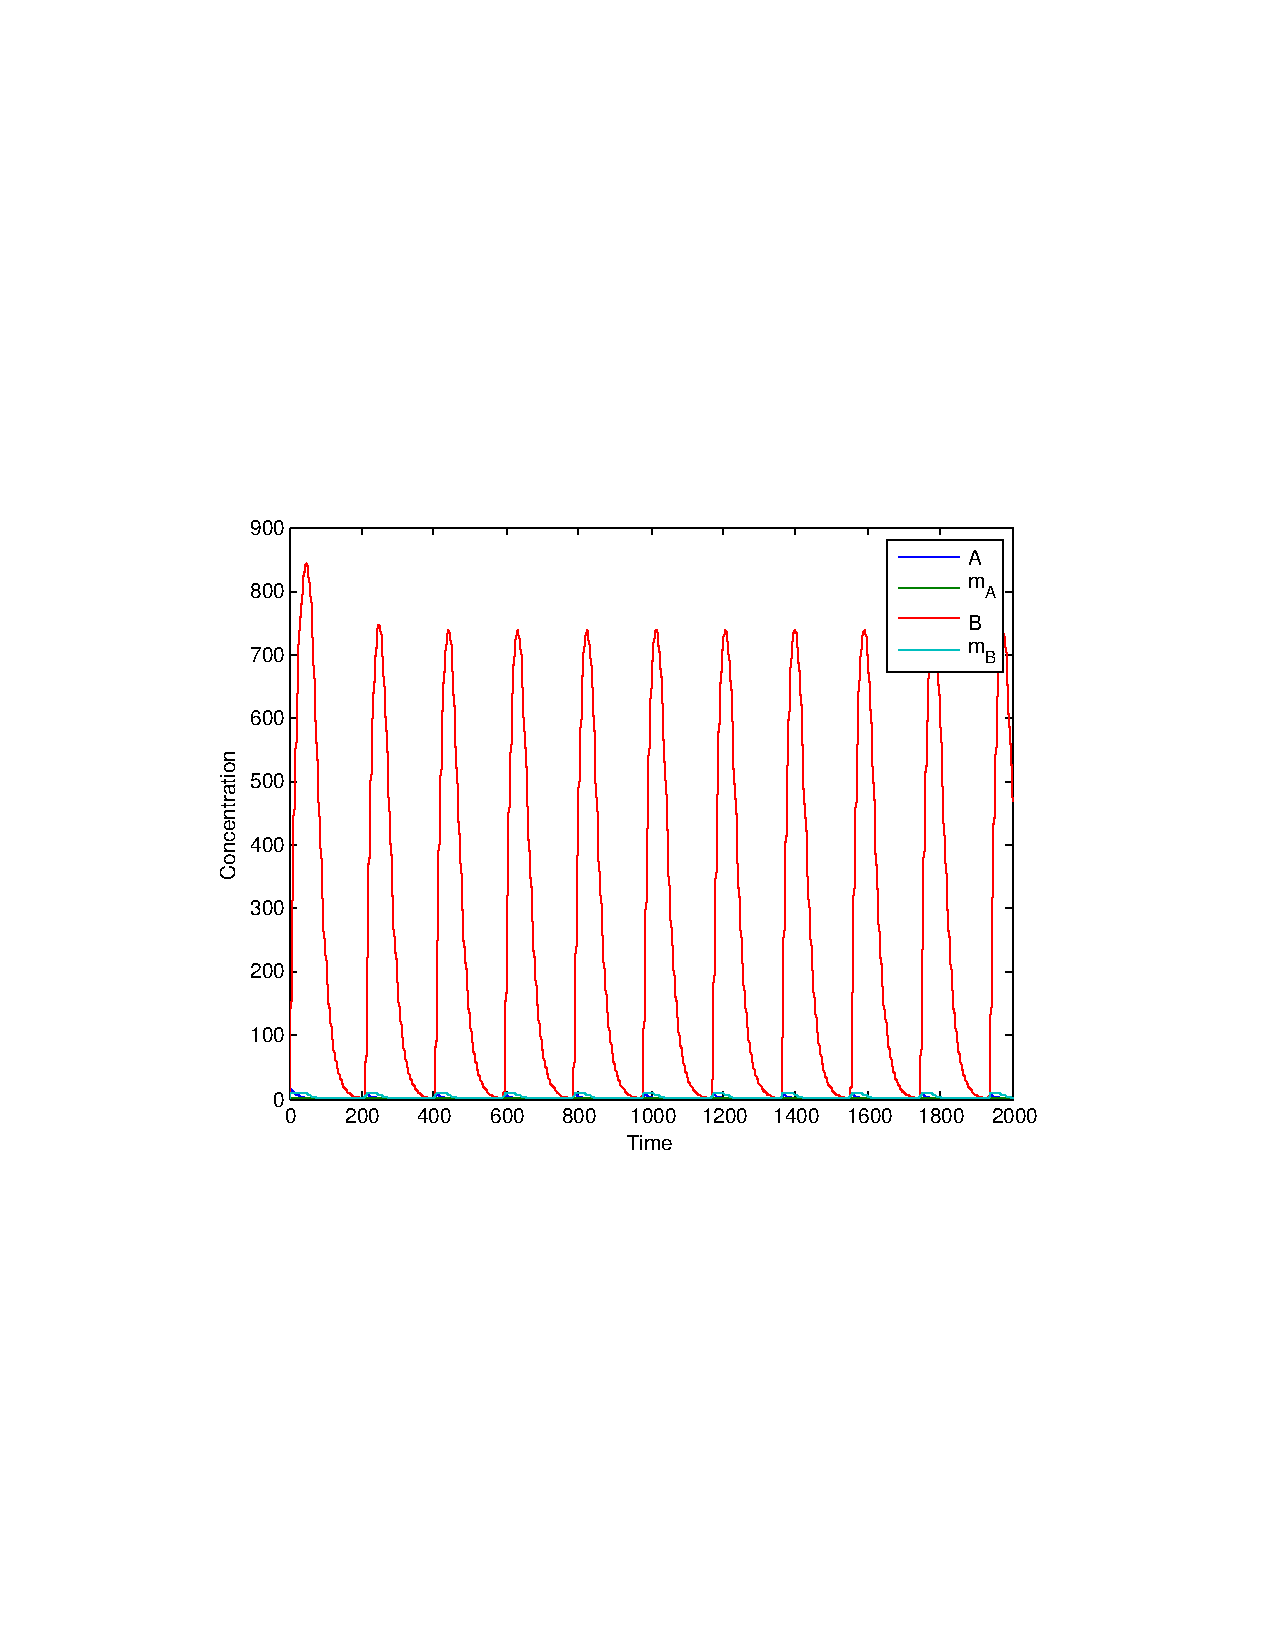
\includegraphics[scale=0.60, clip=true, trim=3.5cm 8cm 3.5cm 8cm]{sys3.pdf}
\end{figure}

\end{frame}

\begin{frame}{A tasty treat for suffering through these slides}

\href{http://vimeo.com/37189162}{http://vimeo.com/37189162}

\emph{A microfluidic device is filled with bacteria that express a synchronized oscillator circuit. The cells are constantly dividing and are washed away at the bottom to make room. Synchronization is achieved using a small diffusible molecule.}

\vspace{3 mm}

\href{http://vimeo.com/33812959}{http://vimeo.com/33812959}

\emph{A set of microfluidic devices share the same air and are furthermore coupled using $H_2O_2$.}

Prindle \emph{et al.} A sensing array of radically coupled genetic 'biopixels'. Nature 2012, \href{http://go.nature.com/lrOtKQ}{http://go.nature.com/lrOtKQ}


\vspace{3 mm} \pause

\textbf{Modeling} helped figure out the right conditions for getting these oscillations!

\end{frame}

\end{document}